\section{Preliminary work}
\label{sec:preliminary_work}

\subsection{Intuition}
\begin{figure}
	\centering
		
	\hfill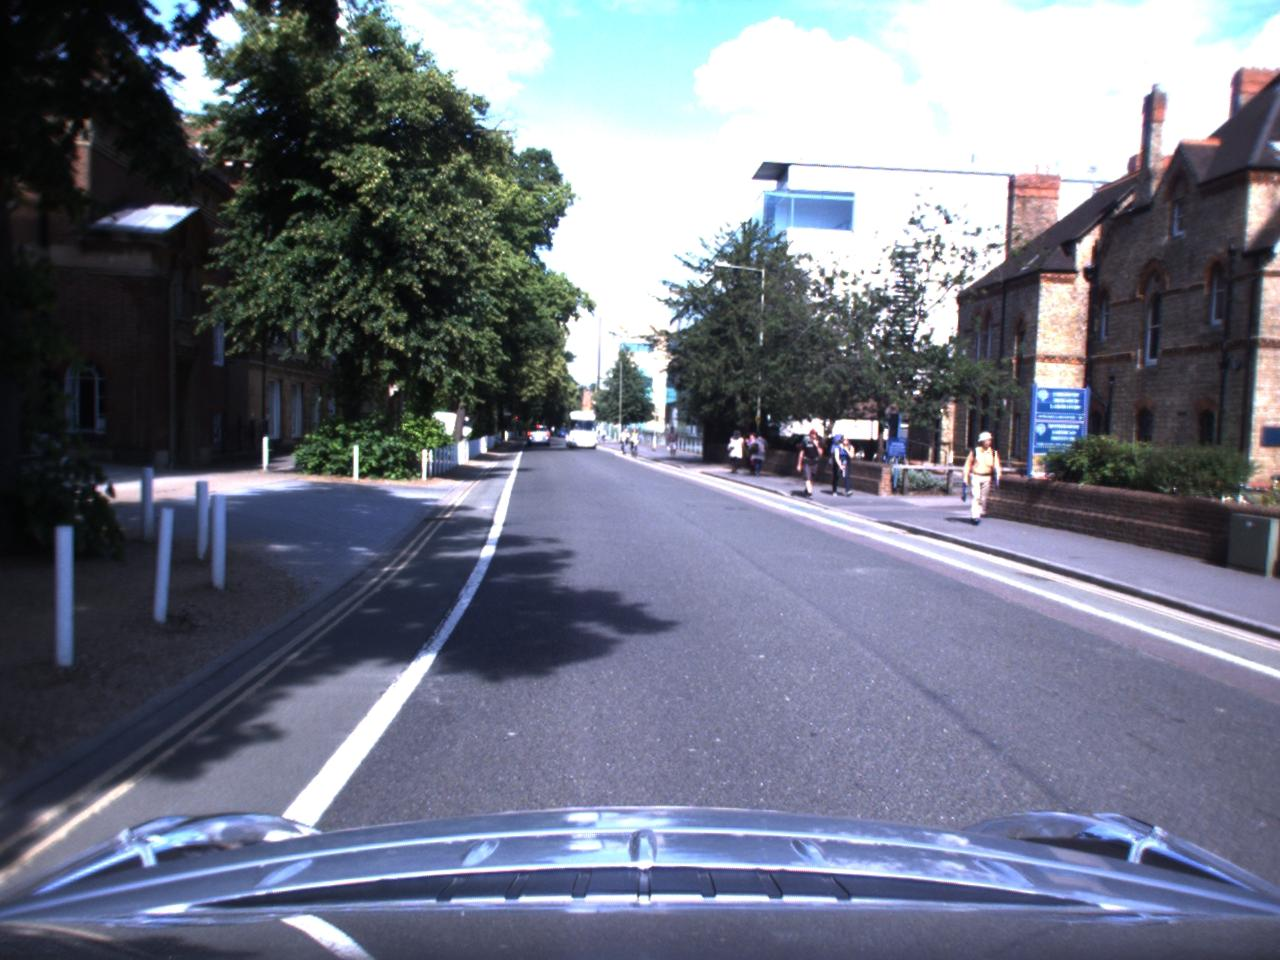
\includegraphics[width=0.25\linewidth]{preliminary/sun}\hfill
	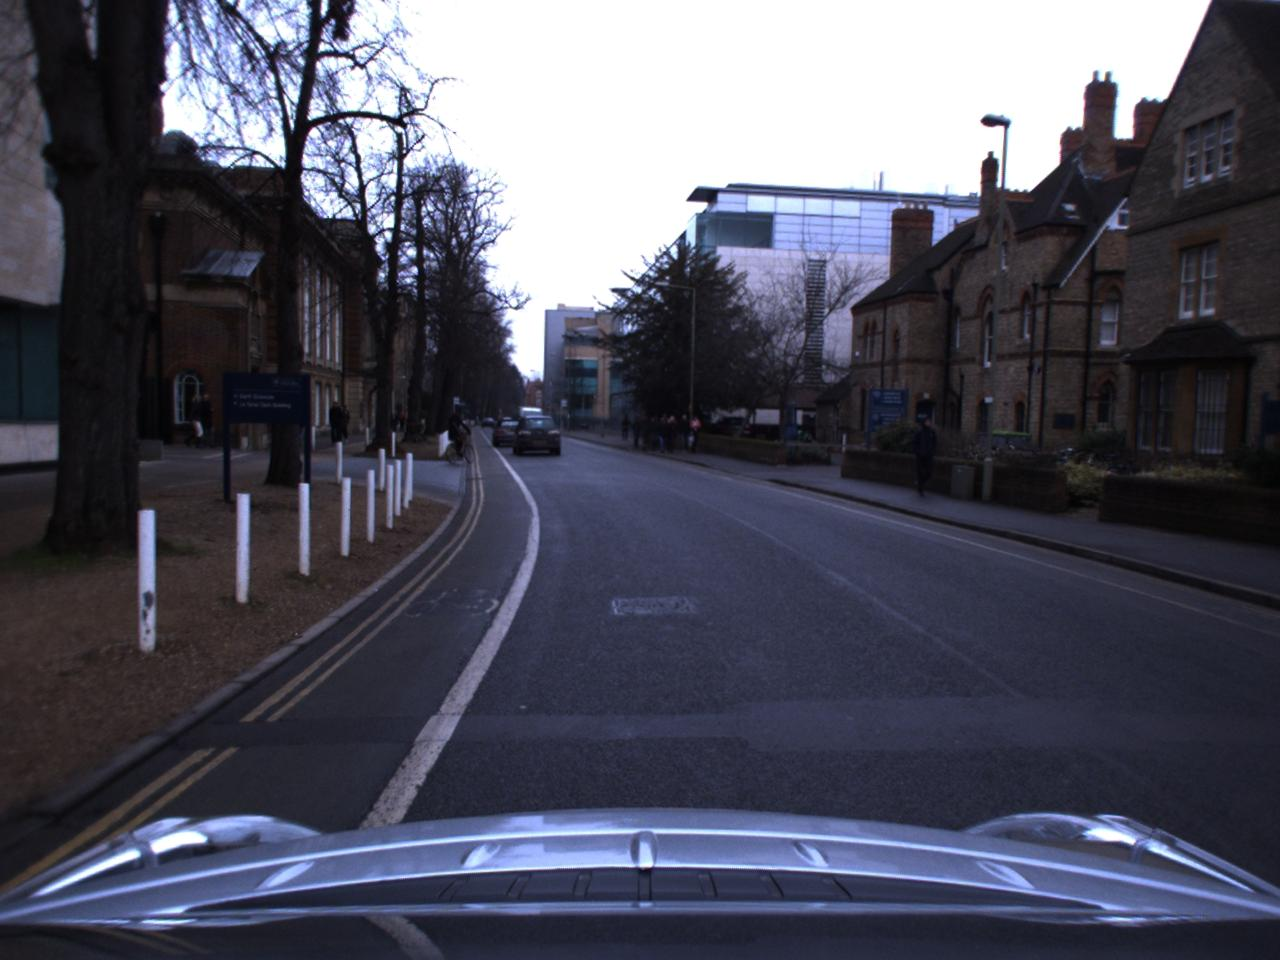
\includegraphics[width=0.25\linewidth]{preliminary/overcast}\hfill
	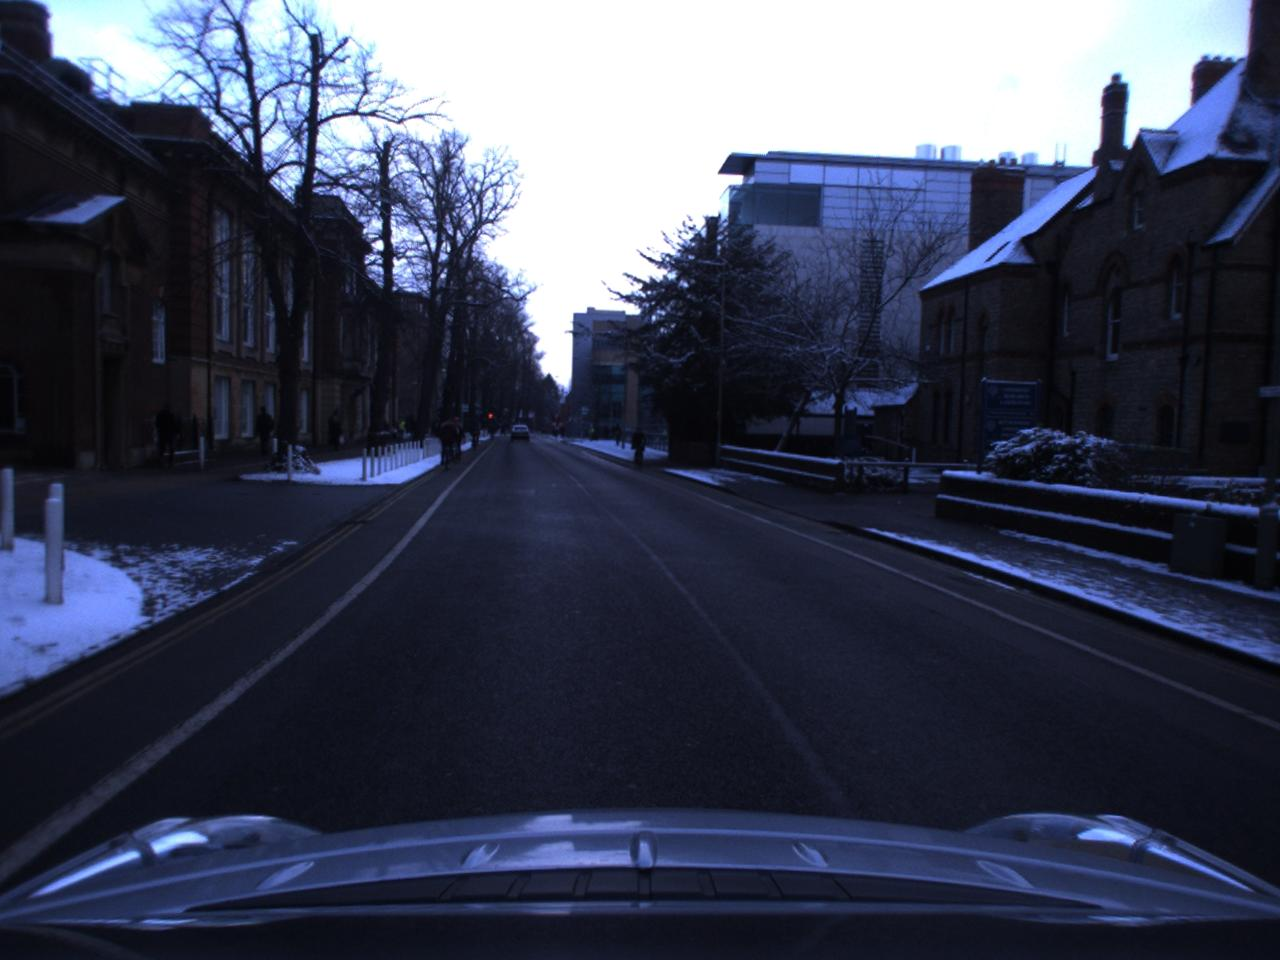
\includegraphics[width=0.25\linewidth]{preliminary/snow}\hfill
	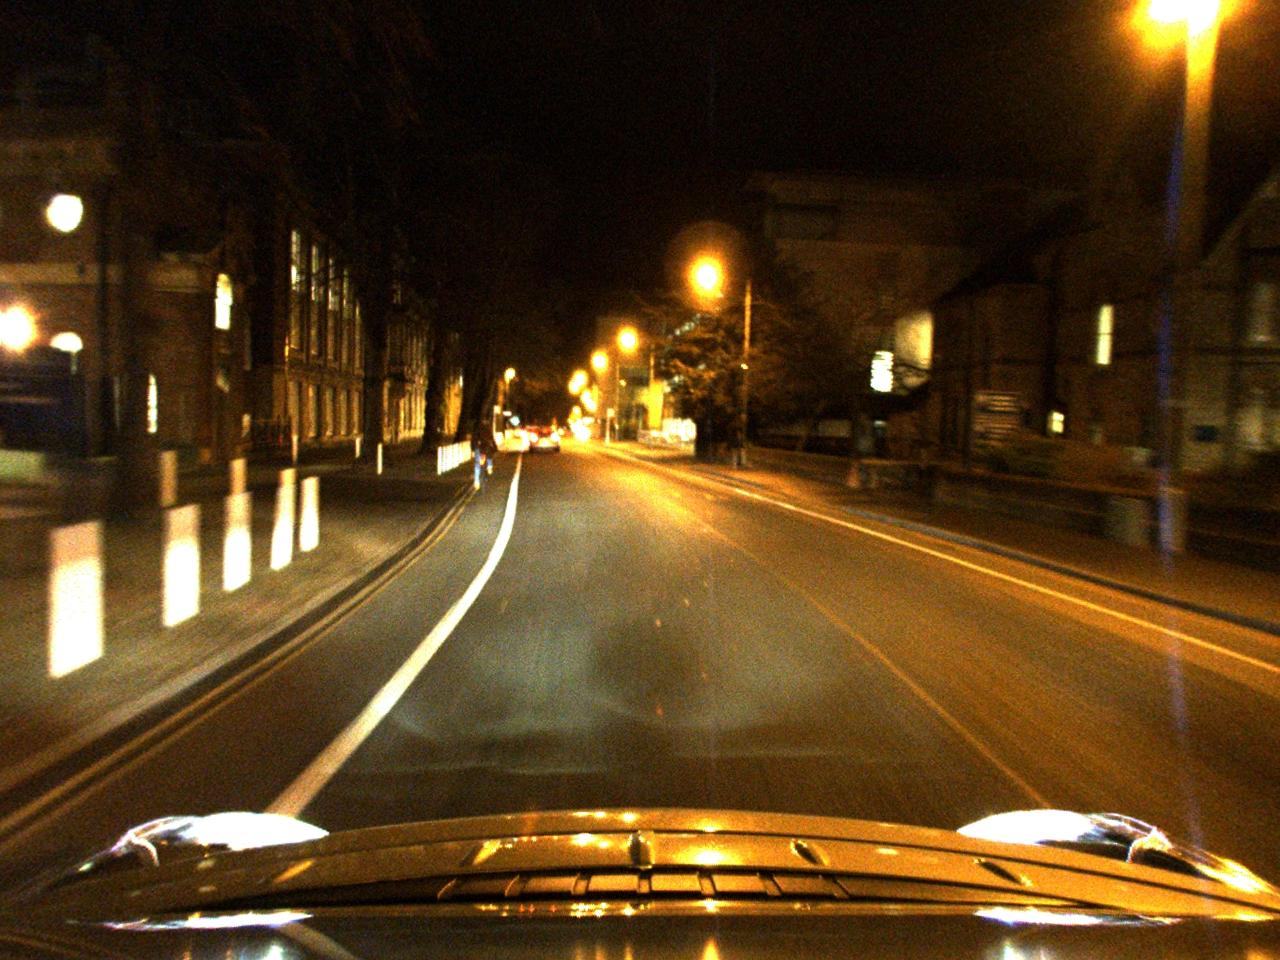
\includegraphics[width=0.25\linewidth]{preliminary/night}\hfill
	
	\hfill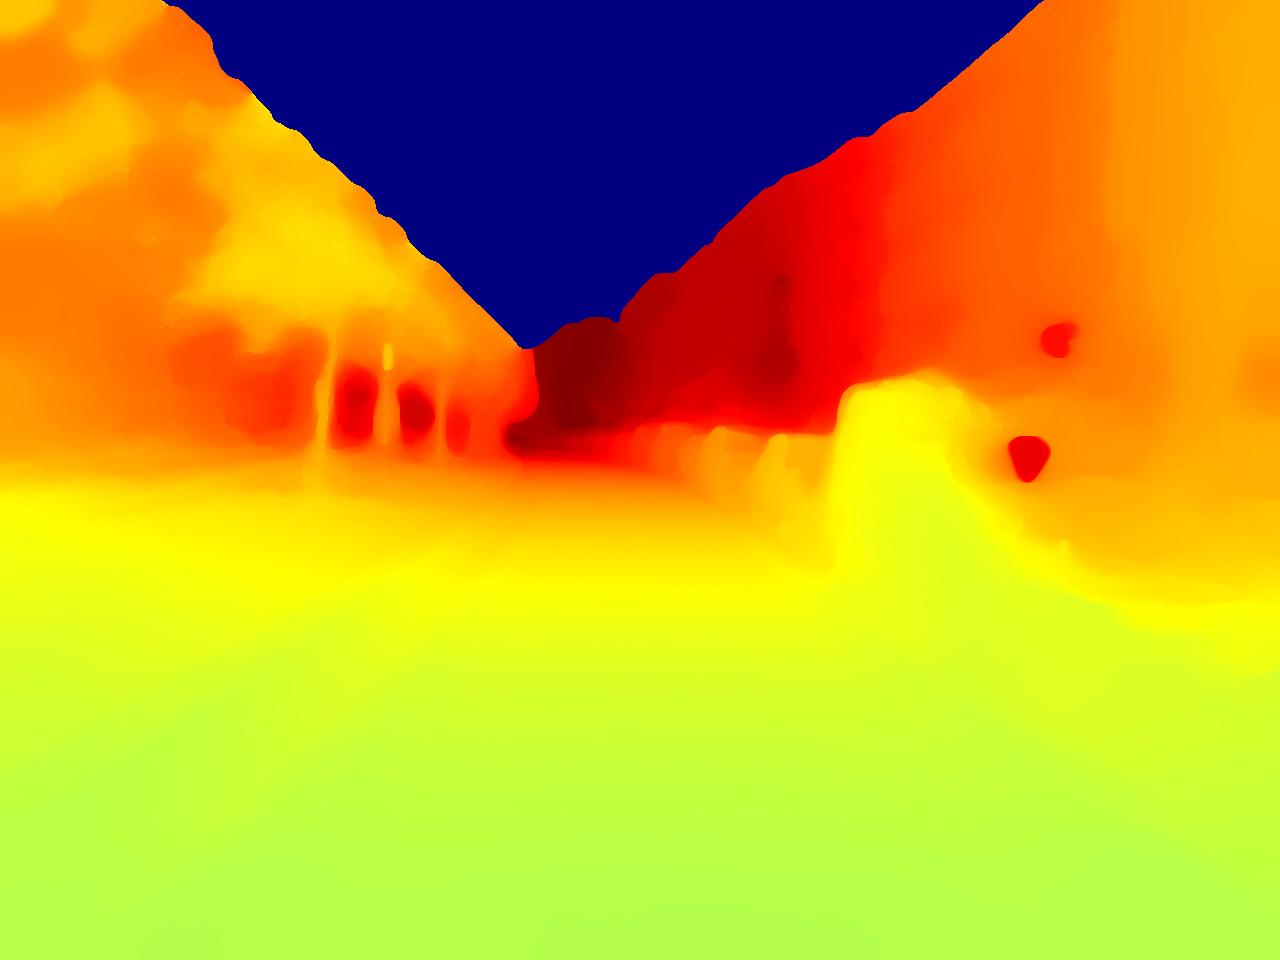
\includegraphics[width=0.25\linewidth]{preliminary/depth}\hfill
	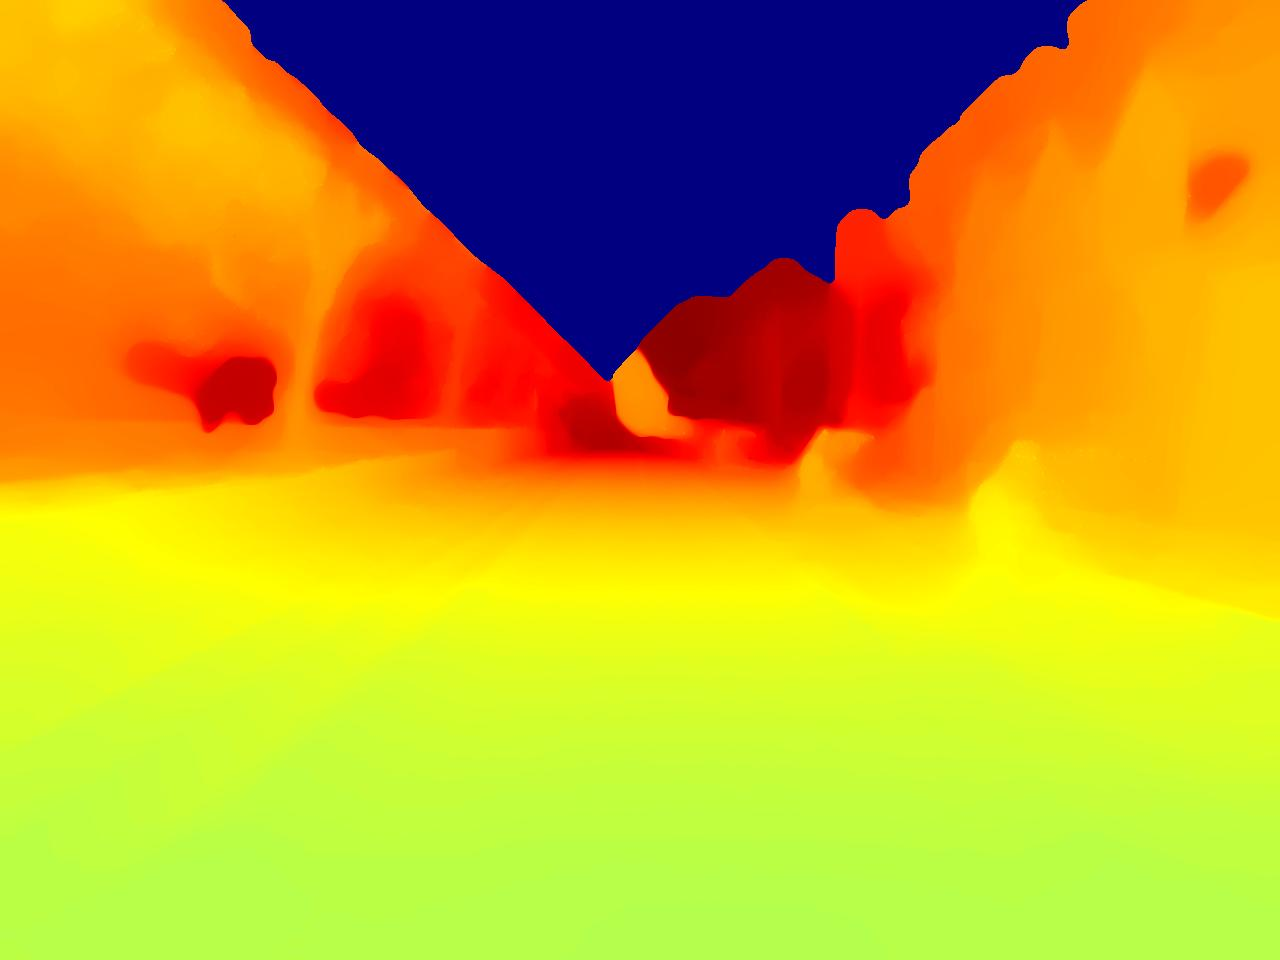
\includegraphics[width=0.25\linewidth]{preliminary/depth3}\hfill
	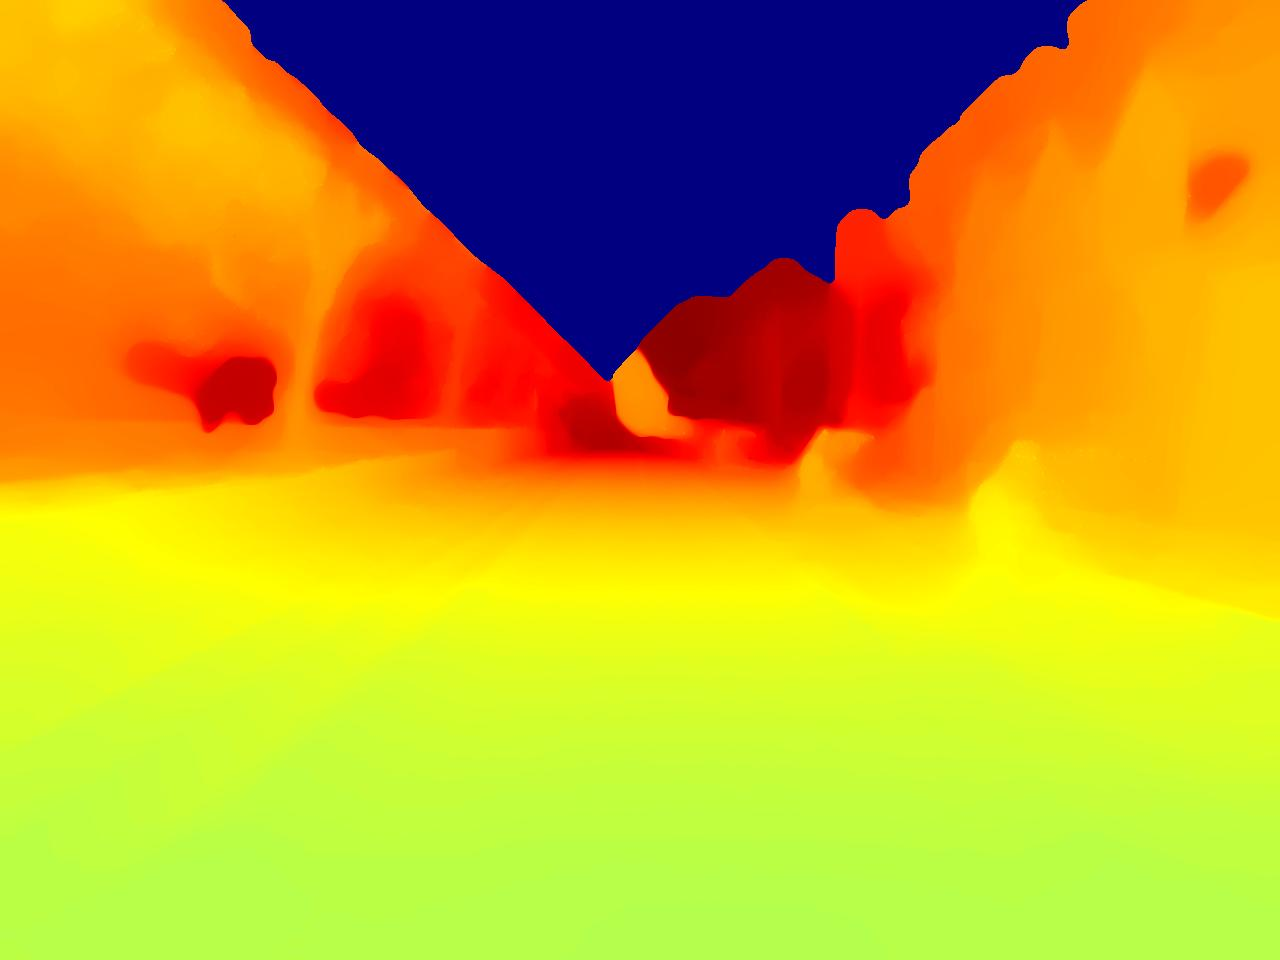
\includegraphics[width=0.25\linewidth]{preliminary/depth3}\hfill
	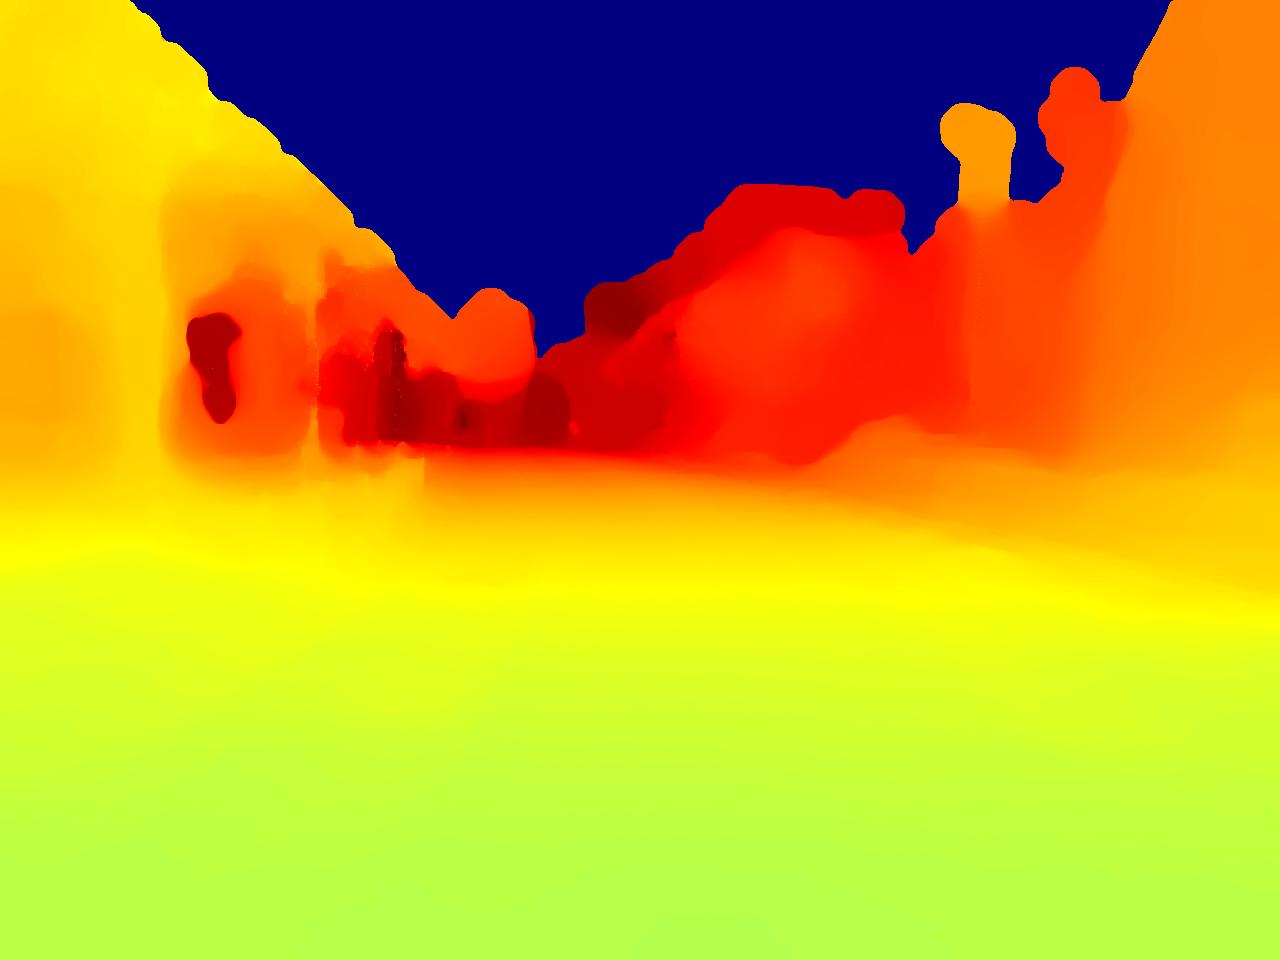
\includegraphics[width=0.25\linewidth]{preliminary/depth4}\hfill

	\caption[Images and depth maps comparison]{\label{fig:image_vs_depth} \textbf{Visual changes between radiometric and geometric domain:} due to outdoor conditions, visual aspect of images changes over time (top row), while, geometry of the scene (corresponding depth maps, bottom row) remains stable.}
	
\end{figure}
	
figure~\ref{fig:image_vs_depth}


\subsection{Method components}
\begin{figure}
	\centering
	
	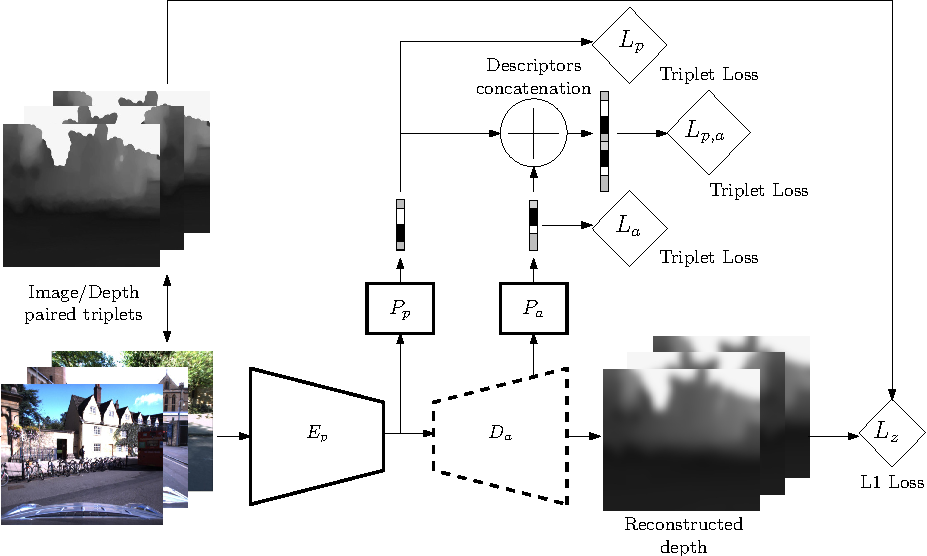
\includegraphics[width=\linewidth]{preliminary/preliminary_method}
	
	\caption[Preliminary solution]{\label{fig:preliminary_method} \textbf{Training pipeline of our preliminary solution.}}
	
\end{figure}
figure~\ref{fig:preliminary_method}

\subsubsection{Descriptor}


\subsubsection{Depth from monocular}



\subsection{Baseline}
\begin{figure}
	\centering
	
	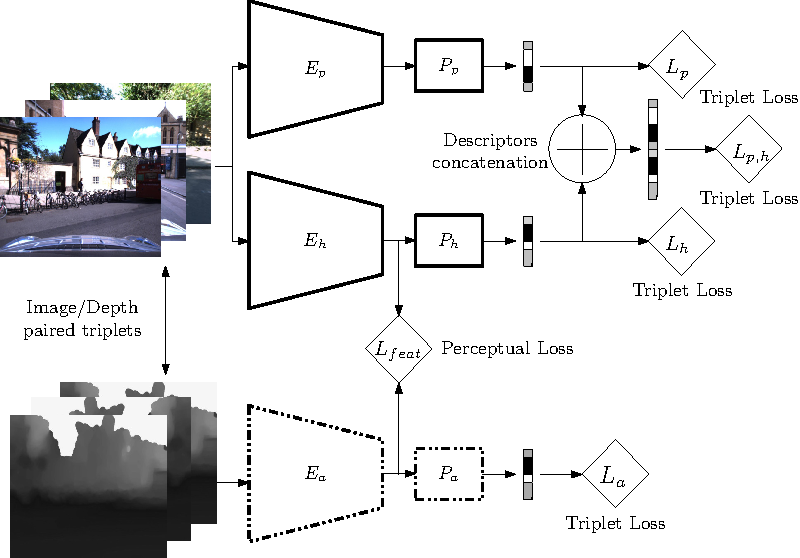
\includegraphics[width=\linewidth]{preliminary/hall_method_training}
	
	\caption[Hallucination network for image descriptors learning]{\label{fig:hall_method} \textbf{Hallucination network for image descriptors learning:} we train an hallucination network, inspired from~\cite{Hoffman2016}, for the task of global image description. Unlike the proposed method (see figure~\ref{fig:our_method}), hallucination network reproduces feature maps that would have been obtained by a network trained with depth map rather than the deep map itself.}
	
\end{figure}
figure~\ref{fig:hall_method}
knowledge distillation~\citep{hinton2015distilling}

We compare our method of side information learning with a state-of-the-art approach system, named hallucination network~\cite{Hoffman2016}. The hallucination network is originally designed for object detection and classification in images. We adapt the work of~\cite{Hoffman2016} to create an image descriptor system that benefits from depth map side modality during training. Like our proposal, the trained hallucination network is used on images only and produces a global descriptor for image localization. The system is presented in figure~\ref{fig:hall_method}. The main difference with our proposal is that the hallucination network reproduces feature maps that would have been obtained by a network trained with depth map rather than the depth map itself. We refer readers to~\cite{Hoffman2016} for more information about the hallucination network.

\subsection{Preliminary results}

